\subsection{Gradient Descent Methods for Linear Regression}
We tested 4-5 different fixed (constant) learning rates. The full plot of these are in the appendix. We found that the best one was X, so we use X when we compare plain GD and plain GD with momentum as well as the analytical solution in figure \ref{fig:plainVSanalytical}.
\begin{figure}
    \centering
    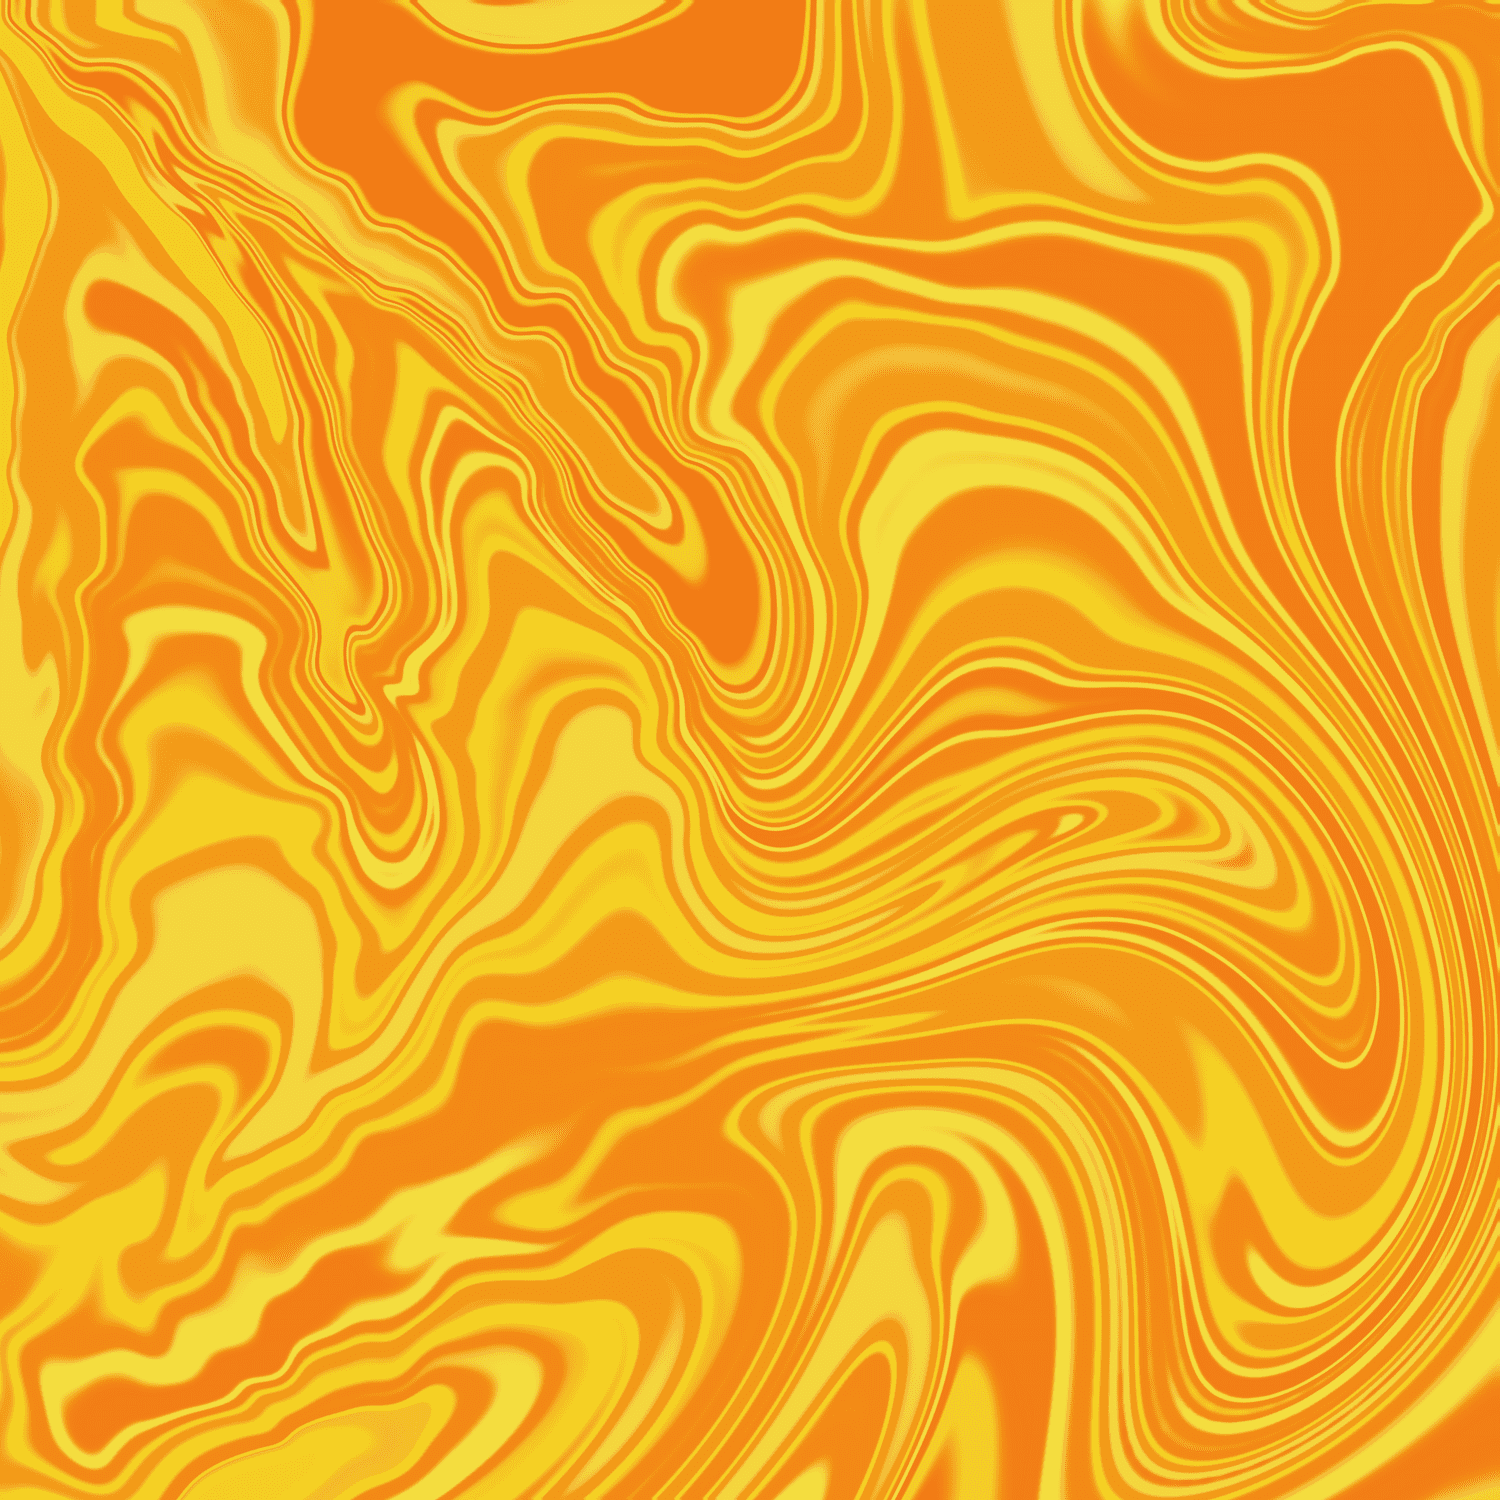
\includegraphics[width=0.5\linewidth]{figures/placeholders/plainVSanalytical.png}
    \caption{\textcolor{purple}{Plot showing our plain GD, plain GD with momentum compared to analytical solutions. Function of iterations.}}
    \label{fig:plainVSanalytical}
\end{figure}

Next, we tested SGD and SDG with momentum with crude tunable learning rate (changes with iteration t). The linearly decaying learning rate expression used in this case was \textcolor{red}{(choose parameters and update equation below.)}:
\[
\eta_t = (1- \kappa)\eta_0 + \kappa \eta_\tau 
\]
Our tests shows the best mini-batch size was X, so we kept this rate fixed and plotted as function of number of epochs. 
\begin{figure}
    \centering
    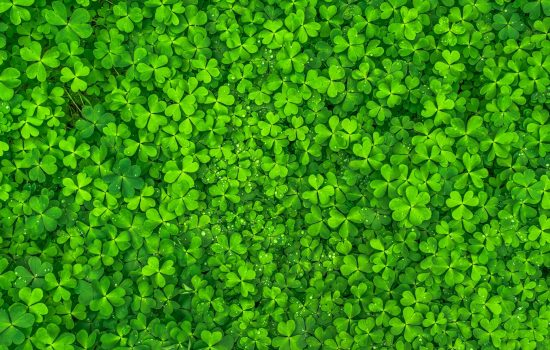
\includegraphics[width=0.5\linewidth]{figures/placeholders/sgdVSanalytical.png}
    \caption{\textcolor{purple}{Plot showing our SGD, SGD with momentum  compared to analytical solutions, fixed mini-batch size. Function of number of epochs.}}
    \label{fig:sgdVSanalytical}
\end{figure}
\textcolor{purple}{Plot showing our SGD, SGD with momentum  compared to analytical solutions, fixed mini-batch size. Function of number of epochs.}

From this point on, we will continue using SGD for computational efficiency.

Now we test out the methods with tunable learning rates. We initialize them at the same fixed value X. We will plot the learning rates for each of the tunable methods with and without momentum (see photo on Emma's phone) and see if the learning rates are adaptable in the way we intended.\\
\textcolor{purple}{Figure: Plot of 3 subplots showing SGD w and w/o momentum for each of the three methods of adaptable learning rates.  Function of number of epochs.}


Now we will make the same three subplots with MSE. We expect the MSE to be more jittery in the methods without momentum, and also to converge faster.\\
\textcolor{purple}{Figure: Plot of 3 subplots showing SGD w and w/o momentum for each of the three methods of adaptable learning rates.  Function of number of epochs.}

Upon comparison with Autograd we see similar/different performance. Our methods pass testing compared to these methods, so we expect our methods will give quite similar results to Autograd.

Up to this point we have only looked at OLS as a regression method. When we use ridge regression instead, we also have to consider the hyperparameter $\lambda$. We will now perform a gird search to find the best possible combination of method and $\lambda$. The grid search table might go in the appendix, but we will state the results here.\\
\textcolor{purple}{Possible figure: Grid search table of the seven possible methods compared for different values of the hyperparameter $\lambda$}

\subsection{Neural Network for Numerical Prediction}
At this point we have to choose a gradient descent method to stick to for at least the numerical prediction task (probably Adam). We will comment the fact that we have tested a few different neural networks, and we will show our best performing one compared to OLS and ridge regression, with the best option for each that we determined in the previous section.\\
\textcolor{purple}{Figure: MSE as a function of epochs for OLS, Ridge and neural network (optimal version of all three methods). We also need a sklearn comparison here.}

\textcolor{purple}{Figure: $R^2$ score as a function of epochs for OLS, Ridge and neural network (optimal version of all three methods). We also need a sklearn comparison here.}

Which method is the best? Why? STATE CLEARLY WHAT PARAMETERS HAVE BEEN USED!
%\textcolor{magenta}{Possible plot: MSE as a function of poly degree, for different lambdas (on the legend)}

\subsection{Neural Network for Classification}
\textcolor{purple}{Figure: Heatmap showing the accuracy for the neural net (on the cancer dataset), as a function of hidden layers (1-5) and nodes in each hidden layer (1-10)}


\textcolor{magenta}{Figure: Activation functions. Plot the accuracy of the network (on cancer data) with different combinations of activation functions [leaky relu, relu, only sigmoid, softmax] (although I believe all should have sigmoid in the final layer), as a function of layers. (I think we should have a fixed number of nodes, unless we want to grid search this and choose the best)} \\ 

\textcolor{purple}{Alternative figure to the one above. The same idea, but with the best layer and node size from the first heatmap/a grid search, as a function of epochs. This makes us able to visualize which activation function converges faster. I think this is a better plot} \\
We expect relu to do well, and converge faster. 

\textcolor{purple}{Figure: Accuracy for [SGD (with and without momentum), Adagrad (with and without momentum), RMSprop and Adam] (on the legend) as a function of epochs, with a fixed learning rate}
\\
We expect them to converge, some faster than others. With momentum should converge faster.
\\
\\
\textcolor{purple}{Figure: Confusion matrix for the neural net (on the cancer dataset, counting the number of TP, TN, FN and FP}
\\
We aim to minimize both false positives and false negatives. A false positive means unnecessary distress for the patient and their family, and wasted hospital resources on additional tests. A false negative, however, could be fatal if cancer goes untreated. Therefore, if the confusion matrix shows a high false negative rate, our loss function should be modified to penalize false negatives more heavily.

\subsection{Logistic Regression for Classification}
\textcolor{purple}{Figure: Confusion matrix of the predictions, so we can compare the two classifiers}

\textcolor{magenta}{Should not be in report, but we should print accuracy/cf before and after scaling with the StandardScaler. Expect accuracy to increase. We can just cite on of our previous reports on scaling with StandardScaler}



